\documentclass[12pt]{article}
  
\usepackage[margin=1in]{geometry} 
\usepackage{amsmath,amsthm,amssymb,bm,mathtools,scrextend}
\usepackage{fancyhdr}
\pagestyle{fancy}
\usepackage{hyperref}

\usepackage{graphicx}
\usepackage[most]{tcolorbox}
\usepackage{algpseudocode}
\usepackage{algorithm}
\usepackage{listings}

\newcommand{\expect}[1]{\mathbb{E}\left[#1\right]}
\newcommand{\av}{\mathbf{a}}
\newcommand{\rv}{\mathbf{r}}
\newcommand{\cv}{\mathbf{cv}}
\newcommand{\C}{\mathbf{C}}
\newcommand{\n}{\mathbf{n}}
\newcommand{\q}{\mathbf{q}}
\newcommand{\x}{\mathbf{x}}
\newcommand{\y}{\mathbf{y}}
\newcommand{\z}{\mathbf{z}}
\newcommand{\0}{\mathbf{0}}
\newcommand{\1}{\mathbf{1}}
\newcommand{\I}{\mathbf{I}}
\newcommand{\X}{\mathbf{X}}
\newcommand{\Y}{\mathbf{Y}}

\newcommand{\hdash}{\rule[.5ex]{1.5em}{0.4pt}}

\newcommand{\DTFT}{\xleftrightarrow{\text{DTFT}}}
\newcommand{\DFT}{\xleftrightarrow{\text{DFT}}}
\newcommand{\ZT}{\xleftrightarrow{\text{ZT}}}

\newcommand{\range}{\text{rng}}

\newcommand{\solspace}{\vspace{3mm} \textbf{Your Solution Here!} \vspace{3mm}}

\definecolor{codegreen}{rgb}{0,0.5,0}
\definecolor{codegray}{rgb}{0.5,0.5,0.5}
\definecolor{codepurple}{rgb}{0.58,0,0.82}
\definecolor{codeblue}{rgb}{0,0,0.6}
\definecolor{codered}{rgb}{0.5,0,0}
\definecolor{backcolour}{rgb}{0.97,0.97,0.95}

\lstdefinestyle{pythonStyle}{
    backgroundcolor=\color{backcolour},   
    commentstyle=\color{codegreen},
    keywordstyle=\color{codeblue},
    numberstyle=\tiny\color{codegray},
    stringstyle=\color{codepurple},
    emphstyle=\color{codered},
    basicstyle=\ttfamily\footnotesize,
    breakatwhitespace=false,         
    breaklines=true,                 
    captionpos=b,                    
    keepspaces=true,                 
    numbers=left,                    
    numbersep=5pt,                  
    showspaces=false,                
    showstringspaces=false,
    showtabs=false,                  
    tabsize=2
}

\lstset{style=pythonStyle}

\begin{document}

\lhead{ECE 551}
\chead{PSET 5 - Sampling}
\rhead{\today}
 
\section{Unmatched Sampling (Theory)}
Modified from Fall 2018\\
Let $U,V$ be finite dimensional signal spaces, and let $T: U \rightarrow V$ be some (linear, perhaps) mapping. 
This problem is about restricting the domain of a mapping to allow invertibility.

For a subset $R \subset U$, we denote the \href{https://en.wikipedia.org/wiki/Restriction_(mathematics)}{restriction} of $T$ to $R$ by $T|_R$ (same map, whose domain is now restricted to the subset $R$).
As an example, you may think of sampling bandlimited signals. The sampling operation itself is not inherently invertible, but given the constraint of strictly bandlimited signals, it becomes invertible.

\textbf{(a)} For this part only assume $U = \mathbb{C}^3$. Find a linear map $T: U \rightarrow \mathbb{C}^2$ (naturally non-invertible) and some subspace $R \subset U$ such that the restriction is $T|_R$ invertible.
Prove that your chosen $T$ is indeed invertible on $R$.

\solspace

\textbf{(b)} For your given $T: U \rightarrow V$, determine what are the subspace $R \subset U$ on which $T$ is invertible. 
\textbf{Hint:} Avoid the nullspace of $T$ (the set of vectors $v$ such that $Tv = 0$).

\solspace

Let $\Phi$ and $\tilde \Phi$ be synthesis and sampling operators, both of full rank
\begin{align*}
    \Phi&: \mathbb{C}^M \rightarrow U  &\text{(Synthesis)} \\
    \Phi&: U \rightarrow \mathbb{C}^N  &\text{(Sampling)}
\end{align*}
and assume that $R = \range(\Phi)$ and $S = \range(\tilde \Phi)$ are the ranges of the respective operators. We look for conditions under which signals in $R$ can be fully recovered when sampled by $\tilde \Phi$, that is, there exists $\Psi$ such that
\begin{equation}
    \Psi \tilde \Phi^* x = x \qquad \text{ for all } x \in \mathbb{R},
\end{equation}
or in other words, the restriction $\Psi \tilde \Phi^*|_R$ is an identity.

\textbf{(c)} Show that the condition below is necessary for such recovery:
\begin{equation}
    \null(\tilde \Phi^*) \cap R = \{0\},
\end{equation}
which means that the only $x \in R$ such that $\tilde \Phi^* x = 0$ is $x=0$.\\
What is the implication (in terms of sampling) of this condition ?

Optional: Show that the condition is also sufficient.

\solspace

\textbf{(d)} Let $\tilde \Phi^* = \begin{bmatrix}
    1 & 2
\end{bmatrix}$ and let $\Phi = \begin{bmatrix}
    1 \\ 3
\end{bmatrix}$. Compute the matrix represnetation of the recovery system $\Psi$ (with respect to the standard basis), and $\Psi \tilde \Phi^*$

\solspace

\textbf{(e)} Show that $\Psi \tilde \Phi^*$ is a projection from $U$ to $R$.

\solspace

\pagebreak

\section{Radon Transform (Theory)}
In this section, you will formalize many notions regarding the Radon transform.

\textbf{Q1:}\\
Recall that in lecture, we gave the definition 
\begin{equation}
	(Rx)[n,\theta] = \int_{\ell_{n,\theta}}f(l) dl = \int_{-\infty}^{\infty}f\left(G_\theta\begin{bmatrix}
		n \\ t
	\end{bmatrix}\right) dt
\end{equation}
for the forward operator.
Give one additional form for the operator: express it as a double integral over $x,y$ using a delta function.

\solspace

\textbf{Q2:}\\
Now, we loosely talked about how $R^*$ should spread the measurements back across the image.
Please define the operator mathematically.

\solspace

\textbf{Q3:}\\
There is a well-known theorem relating the Radon Transform and the Fourier Transform. It is very helpful for understanding the pseudoinverse operator.
The following terminology may be confusing because the forward operator is referred to as a projection.

The Fourier transform of a projection of an image (applying $R$ for a fixed angle $\theta$) is equal to the slice of the center of the 2D Fourier transform of the image parallel to the projection plane.

The relevant planes are illustrated in the below figure.
\begin{figure}[h]
    \centering
    
\includegraphics[width=0.4\textwidth]{ProjectionSlice.png}
\end{figure}

If we use $\mathcal{F}_k$ to denote a $k$ dimensional Fourier Transform, then
\begin{equation}
    [\mathcal{F}_2(f)]\left(G_\theta\begin{bmatrix}
        \omega \\ 0
    \end{bmatrix}\right) = 
    \mathcal{F}_1\left(\int_{-\infty}^{\infty}f\left(G_\theta\begin{bmatrix}
		x \\ t
	\end{bmatrix}\right) dt\right),
\end{equation}
where in the above expression, $\omega$ is being used to indicate the frequency index, $x$ is being used to indicate the spatial index, and $\theta$ is setting the direction of the projection.

Hint: First, think intuitively about the meaning of this theorem, there is a nice reason it holds. Then use your expressions from Q1 and Q2. \\
\textit{As a side note from the TA, the description in words and the picture takes priority over equation 4. If the orientation of the slice is incorrect or anything, let me know.
I'm fairly confident in the equation, but it's still possible I messed up the rotation.}

\solspace

\textbf{Q4:}\\
Show that in the under-determined case $(R^* R)^{-1}$ is equivalent to applying an LTI filter.

\solspace

\textbf{Q5:}\\
By using the x-axis as the projection angle, the y-axis as the projection position, and the intensity as the value, sketch the Radon transforms of the following images.
\begin{figure}[h]
    \centering
    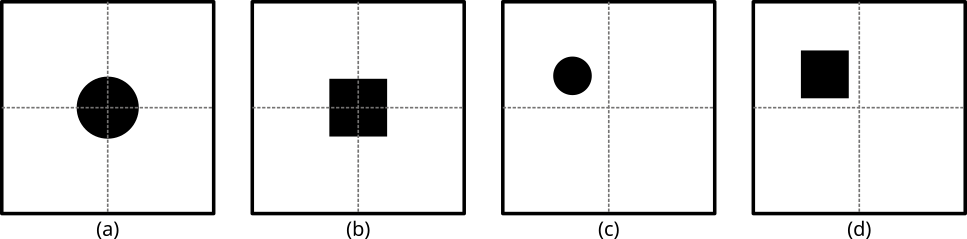
\includegraphics[width=0.9\textwidth]{radonQ.png}
\end{figure}

\solspace

\pagebreak
\section{Multichannel Sampling}
From Spring 2018 Boston University ENG EC 416/516\\

Let $x\in BL[-\pi,\pi]$ and T=1. Consider an N-channel system with sampling prefilters $\tilde g_i, i= 0,1,...,N-1$ followed by uniform sampling with period NT.

\textbf{(a)} Let $N=3$, and let the sampling prefilters be derivative filters: $\tilde G_i(\omega) = (j\omega)^i, i = 0,1,2$. Show that the determinant of the matrix $\tilde G(\omega)$ is a nonzero constant.

\solspace

\textbf{(b)} Let $N \in \mathbb{Z}^+$, and let the sampling prefilters be derivative filters: $\tilde G_i(\omega) = (j\omega)^i, i = 0,1,...,N-1$. Show that the determinant of the matrix $\tilde G(\omega)$ is a nonzero constant.

\solspace

\textbf{(c)} Let $N=3$, and let the sampling prefilters be delay filters: $\tilde G_0(\omega) = 1, \tilde G_1(\omega) = e^{-j\omega(1+\alpha)}, \tilde G_2(\omega) = e^{-j\omega(1+\beta)}$. For which values of $\alpha, \beta \in [-1,1]$ is the matrix $\tilde G(\omega)$ singular? Numerically compute the condition number $\kappa(\tilde G(\omega))$; you should obtain that it does not depend on $\omega$. Plot $\tilde G(\omega)$ for $\alpha = 1$ and $\beta \in [-\frac{1}{2},\frac{1}{2})$. Comment on the results.

\solspace

\pagebreak
\section{Radon Transform (Computation)}
We discussed that in the Radon transform of an image, we take values of the pixels that the particular line passes through.

\textbf{(a)}
Treating the Radon transform as a matrix-vector multiplication, where the vector is the result of $\text{vec}(x)$ and $x$ is the original image, what is an explicit expression for $R_{i,j}$?

\solspace

\textbf{(b)}
Sample and interopolate the Shepp-Logan phantom using the Radon transform and backprojection, both with and without the ramp filtering. Feel free to use
\begin{itemize}
    \item \verb|skimage.transform.rescale| (To downsample the image)\vspace*{-4mm}
    \item \verb|skimage.transform.radon|\vspace*{-4mm}
    \item \verb|skimage.transform.iradon|\vspace*{-4mm}
    \item \verb|skimage.data.shepp_logan_phanton|
\end{itemize}

Vary the number of equally spaced projections, and provide images for $N \in \{4,16,64,256\}$. Describe the quality of the reconstruction.

\solspace

\pagebreak

\section{Unmatched Sampling (Computational)}
From Fall 2018

Consider the signal space $\mathbb{R}^M$ with the synthesis operator $\Phi: \mathbb{R}^K \rightarrow \mathbb{R}^M$
\begin{equation}
    (\Phi u)[m] = \sum_{k=1}^K u_k \cos(2\pi k \frac{m}{M}), \quad 0 \leq m \leq M-1, \quad 0 \leq k \leq K-1.
\end{equation}
Define an analysis operator $\tilde \Phi^*: \mathbb{R}^M \rightarrow \mathbb{R}^N$, where $N \leq M-2$, by
\begin{equation}
    (\tilde \Phi^* x)[n] = \sum_{m=n}^{n+1}x[m], where 0 \leq n \leq N-1
\end{equation}

\textbf{(a)} Construct the synthesis and analysis operators as NumPy matrices of appropriate dimensions, named \verb|Phi| and \verb|tPhi|

\solspace

\begin{lstlisting}[language=Python]
# Your Code Here
\end{lstlisting}

\textbf{(b)} Is matrix multiplication the most efficient way of implementing the analysis operator? If so, explain. Otherwise, implement something faster and compare with the matrix-multiplication implementation in terms of complexity and performance.

\solspace

\textbf{(c)} Compute a matrix \verb|Psi| that recovers a vector $x \in \range(\Phi)$ from its samples $\tilde \Phi^* x$ (assuming that is possible), and show that \verb|Psi| is indeed the (left) inverse of \verb|tPhi|. You may use any \verb|SciPy/NumPy| function (\verb|numpy.linalg.pinv()| might be useful in particular)

\solspace

\pagebreak
\end{document}